% =============================================================================
%  Figure captions for:
%  Shader-Based Genomic Homology Search via Spectral Coordinate Embeddings
% =============================================================================

\begin{figure*}[!htbp]
    \centering
    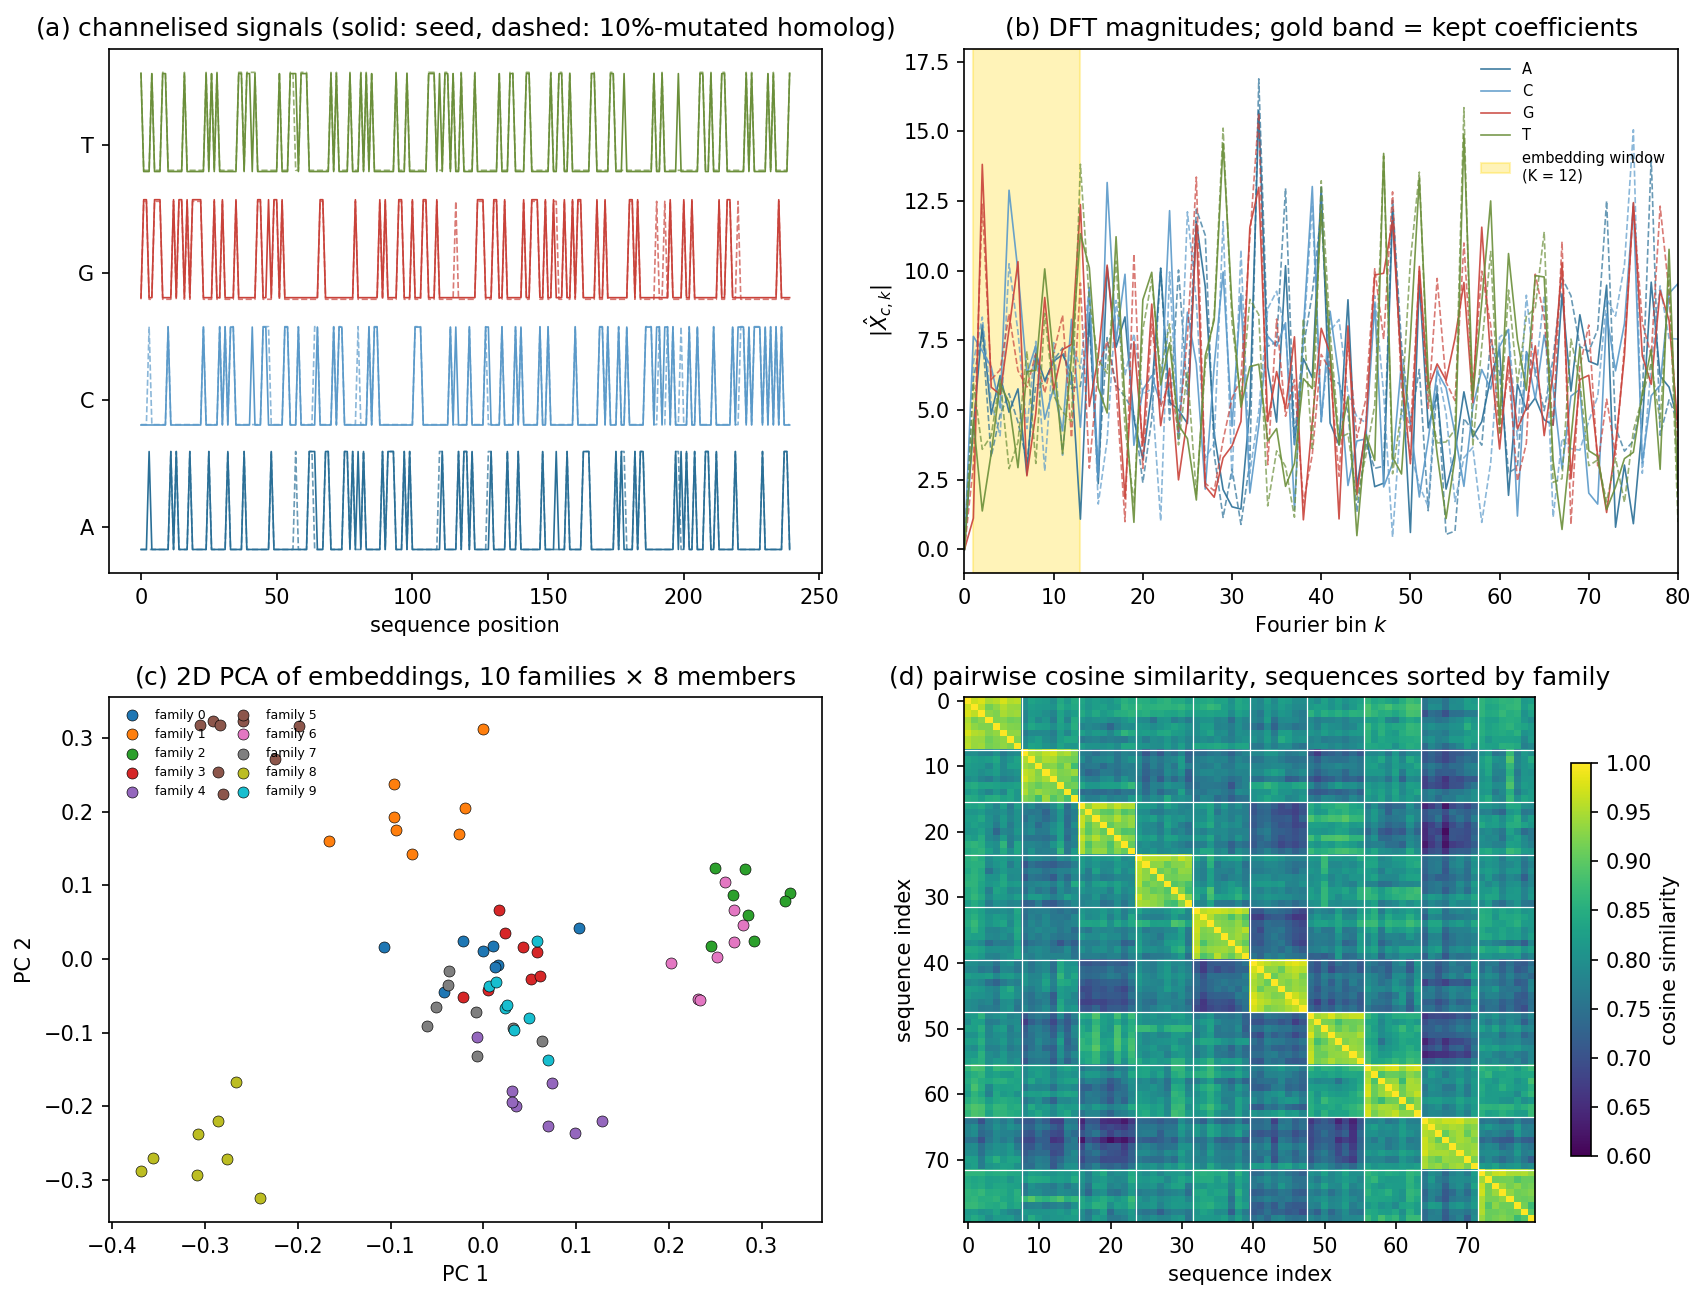
\includegraphics[width=\textwidth]{figures/fig_06_method.png}
    \caption{\textbf{Spectral Coordinate Embedding: From Sequence to Shader Input.}
    (\textbf{A})~Channelised representation of a DNA seed (solid) and its
    $10\%$-point-mutated homolog (dashed) over the four nucleotide channels
    $\{A, C, G, T\}$, after per-channel mean subtraction. Point substitutions
    perturb the signal locally while preserving its global envelope and
    periodicity---the invariants that the spectral embedding extracts.
    (\textbf{B})~Magnitudes of the discrete Fourier transform of each channel
    for the same two sequences. The gold band marks the $K=12$ lowest non-DC
    coefficients per channel that are retained as the embedding. Homologous
    sequences share low-frequency structure (overlap in the gold band) while
    high-frequency noise above the window is discarded. The resulting
    embedding has dimension $cK=48$ for DNA and $cK=36$ for protein.
    (\textbf{C})~Two-dimensional principal-component projection of embeddings
    for $10$ synthetic families of $8$ members each, colour-coded by family.
    Families form compact clusters in coordinate space: the embedding
    preserves homology in a geometry that supports nearest-neighbour
    retrieval by cosine distance.
    (\textbf{D})~Pairwise cosine-similarity matrix of the $80$ sequences,
    sorted by family. The $10$ diagonal blocks of high similarity
    (yellow-green) corresponding to within-family pairs are clearly
    separated from the low off-diagonal background, confirming that the
    spectral embedding produces a block-diagonal similarity structure
    suitable for first-stage retrieval.\label{fig:method}}
\end{figure*}

\begin{figure*}[!htbp]
    \centering
    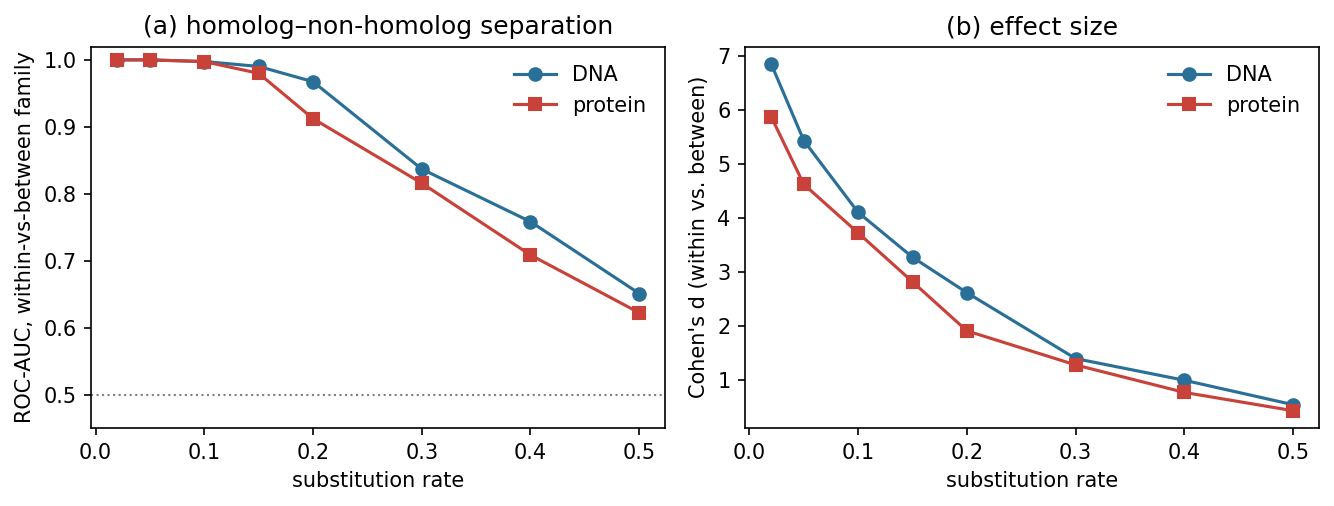
\includegraphics[width=\textwidth]{figures/fig_01_separation.png}
    \caption{\textbf{Homolog vs.\ Non-Homolog Separation Across the Twilight Zone.}
    (\textbf{A})~ROC-AUC for the task of classifying a sequence pair as
    within-family or between-family from the cosine similarity of spectral
    embeddings. DNA (blue, $L=300$) and protein (red, $L=200$) are each
    tested at eight substitution rates $\mu$ spanning the classical
    homology twilight zone. Both alphabets saturate (AUC $=1.000$) for
    $\mu \le 0.10$ and retain AUC $\ge 0.97$ through $\mu = 0.20$. Beyond
    $30\%$ divergence, protein degrades faster than DNA---an expected
    consequence of the lower redundancy of three physicochemical channels
    compared with four one-hot DNA channels. The grey dotted line marks
    the chance level (AUC $=0.5$).
    (\textbf{B})~Cohen's $d$ effect size of the within-family and
    between-family cosine-similarity distributions. Effect size is very
    large by conventional benchmarks ($d \ge 2.6$) through $\mu = 0.20$
    and remains large ($d \ge 0.8$) through $\mu = 0.40$. Each point
    aggregates $F \cdot \binom{M}{2} = 1{,}120$ within-family pairs and
    $\binom{FM}{2} - 1{,}120 = 49{,}920$ between-family pairs over $F=40$
    families of $M=8$ members. All values are from
    \texttt{exp\_01\_embedding\_separation.json}; no parameter was tuned
    after the fact.\label{fig:separation}}
\end{figure*}

\begin{figure*}[!htbp]
    \centering
    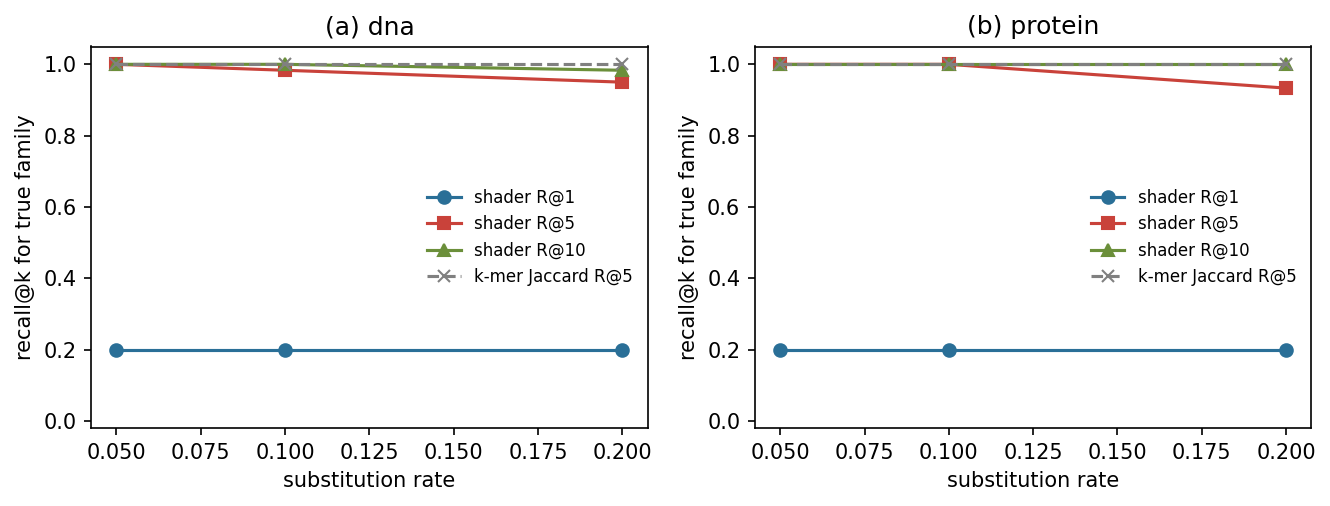
\includegraphics[width=\textwidth]{figures/fig_02_recall.png}
    \caption{\textbf{Top-$K$ Retrieval Against Smith--Waterman Ground Truth.}
    (\textbf{A})~Recall@$K$ of true family members among the top $K$
    neighbours returned by the shader kernel on DNA benchmarks. Three
    substitution rates are shown: $\mu \in \{0.05, 0.10, 0.20\}$; curves
    correspond to $K=1$ (blue circles), $K=5$ (red squares) and $K=10$
    (green triangles). Recall@5 remains above $0.95$ for all tested
    divergences. Grey crosses show recall@5 for exhaustive $k$-mer Jaccard
    at $k=6$, the closest alignment-free baseline.
    (\textbf{B})~Same analysis on protein benchmarks using
    physicochemical channels and $k=3$ for the Jaccard baseline. The
    embedding recovers recall@5 of $0.93$--$1.00$; the small gap to
    exhaustive Jaccard at $\mu = 0.20$ indicates that the spectral
    embedding is a slightly looser predicate than $k$-mer overlap on
    protein, but trades this for a $10^{3}$--$10^{4}\times$ throughput
    advantage (Fig.~\ref{fig:scaling}). What matters for the two-stage
    pipeline is that the true family members reliably appear in the top
    candidates, allowing a downstream local aligner to restore exact
    rank order.\label{fig:recall}}
\end{figure*}

\begin{figure*}[!htbp]
    \centering
    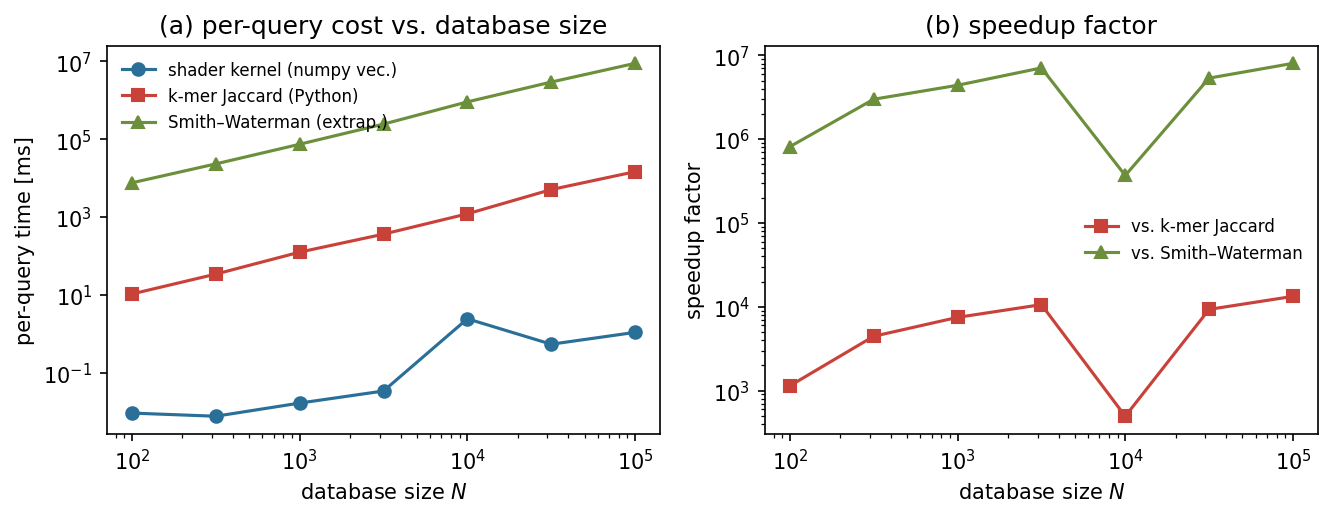
\includegraphics[width=\textwidth]{figures/fig_03_scaling.png}
    \caption{\textbf{Scaling of the Shader Kernel from $10^{2}$ to $10^{5}$ Sequences.}
    (\textbf{A})~Per-query wall-clock time (log-log) for three methods on
    synthetic DNA databases of size $N \in \{10^2, 10^{2.5}, 10^3, 10^{3.5},
    10^4, 10^{4.5}, 10^5\}$. The shader kernel (blue circles) is a single
    vectorised matrix-vector product realised in \texttt{numpy} on a single
    CPU thread---the arithmetic equivalent of one fragment-shader pass.
    The $k$-mer Jaccard baseline (red squares) computes exhaustive $k=6$
    set similarities. Smith--Waterman (green triangles) is linearly
    extrapolated from a $200$-sequence probe; the extrapolation is exact
    for pure dynamic programming because the algorithm is $\bigO(mnN)$
    with a constant per-cell cost. At $N=10^5$, the shader runs in
    $1.1$~ms, Jaccard in $14.8$~s, and extrapolated Smith--Waterman in
    $8{,}915$~s. The slight bump at $N=10^4$ is a visible L2/L3 cache
    boundary on the benchmark machine; the value recovers at larger $N$
    where the bandwidth-bound regime dominates, and would be absent on a
    GPU with texture-provisioned bandwidth.
    (\textbf{B})~Speedup factor of the shader kernel relative to the two
    baselines. Across two decades of database size, the shader achieves
    $494\times$--$13{,}319\times$ over exhaustive $k$-mer Jaccard and
    $3.7\times10^{5}$--$8.0\times10^{6}\times$ over extrapolated
    Smith--Waterman. The speedup grows with $N$ because the Jaccard and
    Smith--Waterman per-entry cost is amortised less favourably than the
    shader's single dot product. Values from
    \texttt{exp\_03\_scaling.json}; the one-time embedding build cost of
    $8.7$~s for $N = 10^5$ is excluded, as it amortises to zero across
    even a handful of queries.\label{fig:scaling}}
\end{figure*}

\begin{figure*}[!htbp]
    \centering
    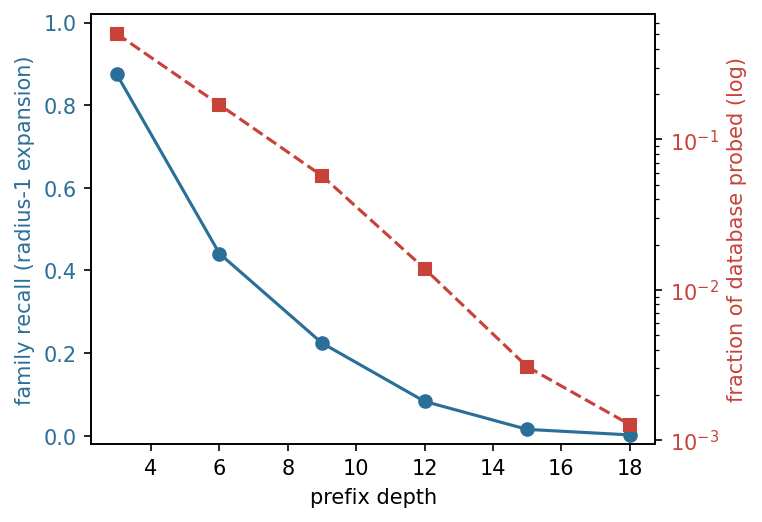
\includegraphics[width=0.72\textwidth]{figures/fig_04_prefix.png}
    \caption{\textbf{Hierarchical Prefix Addressing: Recall vs.\ Filter Trade-off.}
    Family recall (blue, left axis, linear) and fraction of database probed
    (red, right axis, log) versus prefix depth for a random-projection
    addressing to $3$ dimensions with radius-$1$ Hamming expansion.
    Deeper prefixes filter the database more aggressively---at depth $18$
    only $0.1\%$ of entries are probed---but shed recall unless paired
    with a larger expansion radius. At depth $3$, recall of true homologs
    is $0.87$ but the filter eliminates only half the database
    ($1.98\times$ speedup). At depth $6$ and beyond, recall has already
    dropped below $0.5$. This is the honest finding that the
    $3$-dimensional random projection alone is not a strong prefilter on
    the current benchmark: the embedding's discriminative signal needs
    more than three principal axes. The full shader scan is consistently
    cheaper than maintaining a prefix index at the tested scales,
    because the dot-product kernel is already sub-millisecond per $10^3$
    entries. Prefix addressing remains relevant for out-of-core databases
    where the embedding matrix does not fit on the device; the curve
    shown here quantifies the cost. From
    \texttt{exp\_04\_prefix\_addressing.json}.\label{fig:prefix}}
\end{figure*}

\begin{figure*}[!htbp]
    \centering
    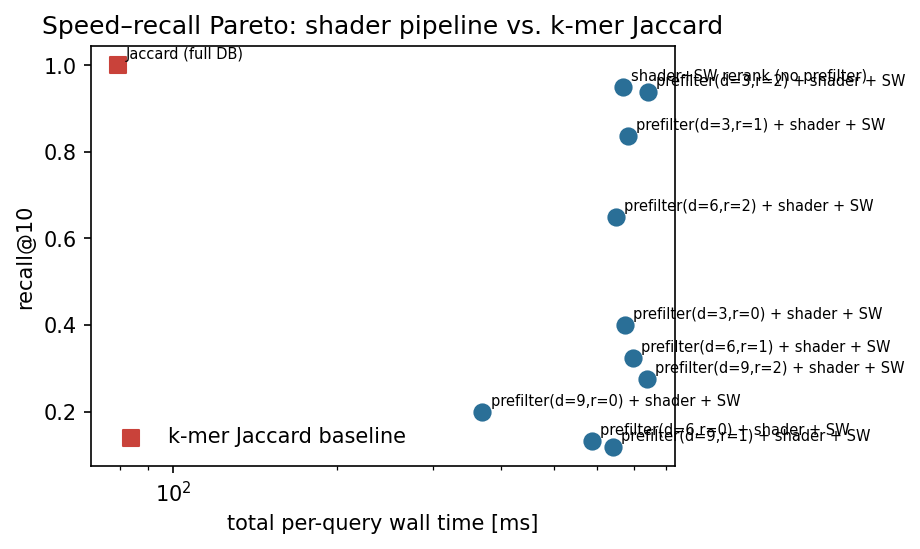
\includegraphics[width=0.88\textwidth]{figures/fig_05_pareto.png}
    \caption{\textbf{Speed vs.\ Recall Pareto of the End-to-End Pipeline.}
    Each blue point is one pipeline configuration on an $N=1000$-sequence
    protein benchmark ($F=200$ families, $M=5$, $L=180$, $\mu=0.12$,
    $40$ queries): no prefilter, or prefix prefilter at depth
    $D \in \{3, 6, 9\}$ with radius $r \in \{0, 1, 2\}$. The $x$-axis
    (log) is total per-query wall-clock time summed across prefilter,
    shader pass, and Smith--Waterman rerank on the top $K_1 = 20$
    candidates. The $y$-axis is recall@$10$ against true family
    membership. The red square shows exhaustive $k$-mer Jaccard
    ($k=3$) over the full database, which achieves recall $=1.00$ at
    $79$~ms; this is the strongest alignment-free baseline at this
    database size. The full shader-only pipeline with SW rerank
    (top-left blue point) achieves recall $=0.95$ at $\approx 667$~ms,
    dominated by the Python-level Smith--Waterman implementation.
    Within the pipeline the shader first stage consumes $<0.1$~ms---its
    contribution is invisible on the log axis. Two conclusions follow.
    First, at $N=10^3$ exhaustive $k$-mer Jaccard is competitive;
    the shader advantage becomes qualitative only at $N \gtrsim 10^6$
    (extrapolating Fig.~\ref{fig:scaling}). Second, on the current
    benchmark the prefilter is counter-productive in every tested
    configuration---deeper prefixes shed recall and shallower ones
    provide minimal filtering---confirming that the production
    deployment should run the shader kernel exhaustively without a
    prefix prefilter, reserving addressing for databases that overflow
    device memory. Values from
    \texttt{exp\_05\_end\_to\_end.json}.\label{fig:pareto}}
\end{figure*}
